\chapter{Planning - Dynamic Programming}

\textbf{Dynamic Programming} (DP) breaks one problem down into smaller sub-problems in order to solve them. Then, you can combine the solutions of the sub-problem to answer the problem.\\

DP is used for planning within an MDP. This means the method assumes there is full knowledge of the MDP. It is technically not Reinforcement Learning yet, since we don't discover an initially unknown environment. It can be used for both \ \textit{prediction} (the input is the MDP and policy, returns value function) and \textit{control} (input only the MDP, returns optimal policy and value function).

\section{Prediction}

\textbf{Iterative policy evaluation} can be used to perform prediction in an MDP (evaluate how good a policy is). On a high level, it works by backing up the Bellman expectation from the states in which rewards are observed. The pseudocode below shows how the algorithm works.

\begin{algorithm}[H]
\caption{Iterative policy evaluation}
\label{alg:it-pol-eval}
    \begin{algorithmic}
    	\REQUIRE the MDP, policy $\pi$
    	\STATE $i \Leftarrow 0$, $v_0(s) \Leftarrow 0$ for each state $s$
        \WHILE{not converged}
        	\FOR{\textbf{each} state $s$}
        		\STATE $v_{i+1}(s) \Leftarrow 
        		\sum_{a \in A} \pi(a|s) \left(R^a_s + \gamma \sum_{s^\prime \in S} P^a_{ss^\prime} v_i(s^\prime) \right)$
        	\ENDFOR
        	\STATE $i \Leftarrow i + 1$
        \ENDWHILE
        \RETURN $v_i$
    \end{algorithmic}
\end{algorithm}

When this algorithm converges, we have obtained the value function $v_\pi$.

\section{Control}

Now that we have a way to evaluate how good a certain policy is, we can start improving it. There are two main ways of performing control using DP. The first method that will be discusses is called \textbf{Policy Iteration}.\\

At each iteration, this method consists of two components: \textbf{policy evaluation} and \textbf{policy improvement}. The whole algorithm works in the following way

\begin{algorithm}[H]
	\caption{Iterative policy evaluation}
	\label{alg:it-pol-eval}
	\begin{algorithmic}
		\REQUIRE the MDP, policy $\pi$
		\WHILE{not converged}
			\STATE $v^\pi \Leftarrow$ iterative policy evaluation with $\pi$
			\STATE $\pi^\prime \Leftarrow greedy(v_\pi)$
			\STATE $\pi = \pi^\prime$
		\ENDWHILE
		\RETURN $v_\pi$, $\pi$
	\end{algorithmic}
\end{algorithm}

The image below shows how this algorithm works on a higher level.

\begin{figure}[H]
	\centering
	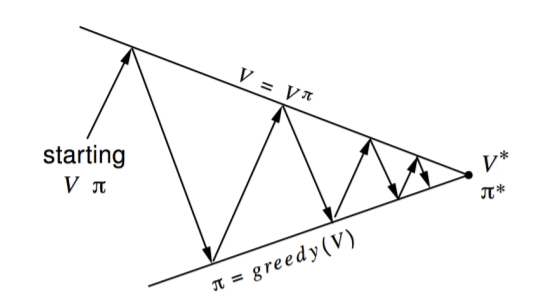
\includegraphics[width=8cm]{policy-iteration}
	\caption{Policy Iteration}
	\label{img:policy-iteration}
\end{figure}

Why does acting greedily with respect to the obtained $v_\pi$ improve the policy? There is a relatively simple proof for this. Say we choose a deterministic policy $\pi(s)$. Acting greedily would mean we create a new policy $\pi^\prime(s) = \arg \max_{a \in A} q_\pi(s, a)$. This means that $q_\pi(s, \pi^\prime(s)) = \max_{a \in A} q_\pi(s,a) \geq q_\pi(s, \pi(s)) = v_\pi(s)$. So we know $q_\pi(s, \pi^\prime(s)) \geq v_\pi(s)$. Therefore, $v_{\pi^\prime}(s) \geq v_\pi(s)$.\\

This means if the improvement stops, we must have satisfied the Bellman optimality equation.\\

Policy iteration can be generalized. Before we performed policy evaluation until we obtained $v_\pi$. However, this is not necessary. The next DP control algorithm, \textbf{Value Iteration}, is a special variant of policy iteration, updating the policy after every step (so not after it converges to $v_\pi$). You can basically use \textbf{any} policy evaluation and policy improvement algorithm to perform policy iteration.\\

Lets now start talking about Value Iteration. This method works because of the \textit{Principle of Optimality}, which states the following: An optimal policy can be subdivided into two components

\begin{itemize}
	\item An optimal first action $A_*$
	\item An optimal policy from successor state $S^\prime$
\end{itemize}

This means that if we know the solution to $v_*(s^\prime)$, we can find $v_*(s)$ by performing the following one-step lookahead. This is possible due to the Bellman optimality equations.

\begin{equation*}
		v^*(s) = \max_{a \in A} \left( R^a_s + \gamma \sum_{s^\prime \in S} P^a_{ss^\prime} v_*(s^\prime)\right)
\end{equation*}

The intuition is that you can start with the final rewards and work your way backwards. 

\begin{algorithm}[H]
	\caption{Value iteration}
	\label{alg:val-iter}
	\begin{algorithmic}
		\REQUIRE the MDP
		\STATE $i \Leftarrow 0$, $v_0(s) \Leftarrow 0$ for each state $s$
		\WHILE{not converged}
			\FOR{\textbf{each} state $s$}
				\STATE $v_{i+1}(s) \Leftarrow 
				\max_{a \in A} \left(R^a_s + \gamma \sum_{s^\prime \in S} P^a_{ss^\prime} v_i(s^\prime)\right)$
			\ENDFOR
			\STATE $i \Leftarrow i + 1$
		\ENDWHILE
		\STATE $v_* \Leftarrow v_i, \pi_*(s) \Leftarrow \arg\max_{a \in A} R^a_s + \gamma\sum_{s' \in S} P^a_{ss'}v_*(s')$
		\RETURN $v_*, \pi_*$
	\end{algorithmic}
\end{algorithm}

Observe that the policy is extracted by acting greedily with respect to the computed q-values for any state. For any intermediate value functions, this might not be true. These in-between value function might not correspond to any policy.\\

The previously discusses algorithms all share a runtime complexity of $O(n^2m)$ per iteration when computing $v$, $n$ being the number of states and $m$ the number of actions. However, the same process can be applied to compute the q-values. This would be $O(n^2m^2)$ per iteration.

\section{Extensions to DP}

So far all described DP methods are \textit{synchronous}. This means all states are updated in parallel. However, these algorithms can also be implemented in an \textit{asynchronous} manner. Since it uses more updated information, it generally converges a lot faster than the synchronous variant. It is also guaranteed to converge as long as all states are continued to be visited. The following three ideas are simple ideas for asynchronous DP with Value Iteration.

\begin{itemize}
	\item In-place DP
	
	Instead of using different value functions $v_i$ at each iteration, we only use one value function. $v_{i+1}(s) = \max_{a \in A} \left(R^a_s + \gamma \sum_{s^\prime \in S} P^a_{ss^\prime} v_i(s^\prime)\right)$ will then become $v(s) = \max_{a \in A} \left(R^a_s + \gamma \sum_{s^\prime \in S} P^a_{ss^\prime} v(s^\prime)\right)$.
	
	\item Prioritized sweeping
	
	Instead of iterating over all states in one order, it is possible to use the magnitude of Bellman error to guide the selection of the next state to evaluate. This bellman error can be expressed as 
	
	\begin{equation*}
		\left|\max_{a \in A} \left(R^a_s + \gamma \sum_{s' \in S} P^a_{ss'}v(s')\right) - v(s)\right|
	\end{equation*}

	The idea is to backup the state with the largest remaining Bellman error and update the Bellman error of the affected states after. This requires knowledge of the reverse dynamics of the MDP, since we are working backwards. It can be very simply implemented using a priority queue.
	
	\item Real-time DP
	
	The idea here is to only update states that are relevant to the agent. The agent's experience can guide the state selection. So, after each time step, we observe $S_t, A_t$ and $R_{t+1}$. We back-up the state $S_t$ by $v(S_t) = \max_{a \in A} \left(R^a_{S_t} + \gamma \sum_{s^\prime \in S} P^a_{S_{t}s^\prime} v(s^\prime)\right)$.
	
\end{itemize}

The DP approach that was discussed this chapter is already good. It is effective for problems containing millions of states. However, since it uses full-width backups, each successor state and action is considered. For large problems this causes DP to suffer from the curse of dimensionality; the number of states grow exponentially with the number of state variables. As proposed in further chapters, this problem is approached using sample backups.

%TODO: Add something about algorithm convergance